%\documentclass{article}
%\usepackage{tikz}
%\usepackage{amsmath}
%\begin{document}
\noindent
\textbf{Beispiel 1} \\ \\
a) 
	\begin{figure}[h]
		\centering
		\usetikzlibrary{arrows}
\tikzset{
pil/.style={
	->,thick,
	shorten<=2pt,
	shorten>=2pt,}
}
\begin{tikzpicture}[scale=0.75]
\draw (-5,0)--(5,0); %Grundfläche
\draw(-4.5,-0.075)--(-4.25,-0.75)--(-4,-0.075)--(-4.5,-0.075); %Gleitlager
\draw [fill=white]  (-4.25,-0.75) circle [radius=5pt];
\draw(4.5,0)--(4.25,-0.75)--(4,0); %Festlager
\draw [fill=white]  (4.25,-0.75) circle [radius=5pt];

\draw [fill=white] (-3,0) rectangle (3,3);
%Kräfte
\draw [->](0,2)--(0,1);
\draw (0.25,1.5) node {\(f_g\)};
\draw [<-](-4.25,-1.25) -- (-4.25,-2.25);
\draw  (-3.75,-2) node {\(f_{A,y}\)};
\draw [<-](4.25,-1.25) -- (4.25,-2.25);
\draw  (4.8,-1.85) node {\(f_{B,y}\)};
\draw [<-](4.75,-0.75) -- (5.75,-0.75);
\draw  (5.25,-0.5) node {\(f_{B,x}\)};
%\draw [fill=blue] (0,0) arc [start angle=90,end angle=300, radius=10pt];
%\draw  [fill=blue] (0,0) -- (2,0.5);



\end{tikzpicture}
	\end{figure} \\
%\noindent
Um die Kräfte in den Lagern zu bestimmten, stellen wir zuerst das Kräftegleichgewicht und die Momenten Gleichung im Punkt B auf. 
\begin{align*}\label{key}
x&: 0=f_{B,x} \\
y&: 0 = f_A + f_{B,y} -f_g\\
M_B&:0=b f_g-2L \cos(\alpha)  
\end{align*}

\noindent
Formt man nun die Momenten Gleichung nach \(f_A\) um folgt: 
\begin{align*}
f_A = \frac{b f_g}{2L \cos(\alpha)} \qquad f_{B_x}=0 \qquad f_{B,y} = \left(1-\frac{b}{2L \cos(\alpha)}\right) f_g
\end{align*}
\begin{figure}[h]
	\centering
	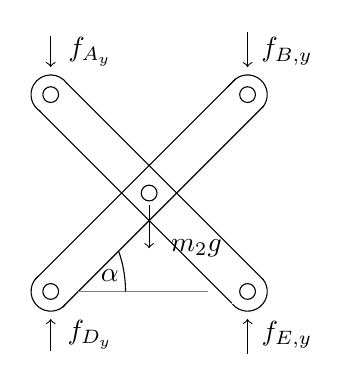
\begin{tikzpicture}[scale=0.5]

\node (v1) at (-2.5,-2.5) {};
\node (v2) at (2.5,2.5) {};
\node (v3) at (0,0) {};
\node (v4) at (-2.5,2.5) {};
\node (v5) at (2.5,-2.5) {};
\draw  (v1) circle (0.2);
\draw  (v2) circle (0.2);
\draw  (v3) circle (0.2);
\draw  (v4) circle (0.2);
\draw  (v5) circle (0.2);
\draw (-2.9,-2.2) -- (2.1,2.8);
\draw (-2.2,-2.9) -- (2.9,2.2);
\draw (-2.117,-2.8214) arc (-40.0022:-230:0.5);
\draw (2.117,2.8214) arc (139.9978:-40:0.5);
\draw (2,2.7) -- (2.2,2.9);
\draw[black!50] (-1.8,-2.5) -- (1.5,-2.5);

\draw (-0.6,-2.5) arc (0:19:3.1);
\draw  (-1,-2.1) node {\(\alpha\)};
\draw (-2.8,2.1) -- (2.1,-2.8);
\draw (-2.1,2.8) -- (2.9,-2.2);
\draw (2.117,-2.8214) arc (-139.9978:40:0.5);
\draw (-2.75,2.067) arc (-120.0007:-325:0.5);
\draw [->](0,-0.3) -- (0,-1.4) ;
\draw (1.2,-1.4) node {\(m_2 g\)};
\draw[<-] (2.5,-3.2) -- (2.5,-4.1);
\draw (3.5,-3.6) node {\(f_{E,y}\)};
\draw [<-](-2.5,-3.2) -- (-2.5,-4);
\draw (-1.5,-3.6) node {\(f_{D_y}\)};
\draw[<-] (2.5,3.2) -- (2.5,4.1);
\draw (3.5,3.6) node {\(f_{B,y}\)};
\draw [<-](-2.5,3.2) -- (-2.5,4);
\draw (-1.5,3.6) node {\(f_{A_y}\)};

\end{tikzpicture}
\end{figure}
b) \\
%\noindent
Um die Kräfte in den Punkten D und E zu bestimmen, stellen wir das Kräftegleichgewicht in den Trägern auf, daraus folgt: 
\begin{align*}
 f_{D,y} = m2 g + f_{B,y}\qquad	f_{E,y} = m_2 g + f_A 
\end{align*}

\begin{figure}[h]
	\centering
	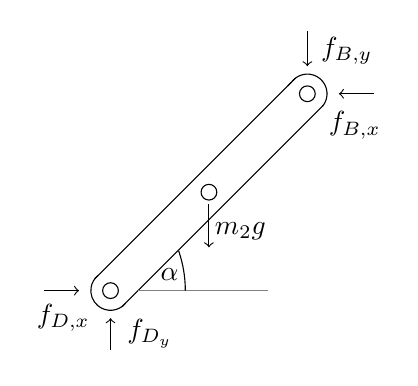
\begin{tikzpicture}[scale=0.5]

\node (v1) at (-2.5,-2.5) {};
\node (v2) at (2.5,2.5) {};
\node (v3) at (0,0) {};
%\node (v4) at (-2.5,2.5) {};
%\node (v5) at (2.5,-2.5) {};
\draw  (v1) circle (0.2);
\draw  (v2) circle (0.2);
\draw  (v3) circle (0.2);
%\draw  (v4) circle (0.2);
%\draw  (v5) circle (0.2);
\draw (-2.9,-2.2) -- (2.1,2.8);
\draw (-2.2,-2.9) -- (2.9,2.2);
\draw (-2.117,-2.8214) arc (-40.0022:-230:0.5);
\draw (2.117,2.8214) arc (139.9978:-40:0.5);
\draw (2,2.7) -- (2.2,2.9);
\draw[black!50] (-1.8,-2.5) -- (1.5,-2.5);

\draw (-0.6,-2.5) arc (0:19:3.1);
\draw  (-1,-2.1) node {\(\alpha\)};
% \draw (-2.8,2.1) -- (2.1,-2.8);
% \draw (-2.1,2.8) -- (2.9,-2.2);
% \draw (2.117,-2.8214) arc (-139.9978:40:0.5);
% \draw (-2.75,2.067) arc (-120.0007:-325:0.5);
\draw [->](0,-0.3) -- (0,-1.4) ;
\draw (0.8,-1.0) node {\(m_2 g\)};
% \draw[<-] (2.5,-3.2) -- (2.5,-4.1);
% \draw (3,-3.6) node {\(f_{D,y}\)};
\draw [<-](-2.5,-3.2) -- (-2.5,-4);
\draw (-1.5,-3.6) node {\(f_{D_y}\)};
\draw[<-] (2.5,3.2) -- (2.5,4.1);
\draw (3.5,3.6) node {\(f_{B,y}\)};
% \draw [<-](-2.5,3.2) -- (-2.5,4);
%\draw (-2.0,3.6) node {\(f_{A_y}\)};



\draw [<-](-3.3,-2.5) -- (-4.2,-2.5);
\draw (-3.7,-3.2) node {\(f_{D,x}\)};
\draw [<-](3.3,2.5) -- (4.2,2.5);
\draw (3.7,1.7) node {\(f_{B,x}\)};
\end{tikzpicture}
\end{figure}
\noindent
c)\\  \\ %\noindent
Um die Kräfte in den Lagern D und E in horizontaler (x-Richtung) zu bestimmen schneiden wir die Hubstangen getrennt voneinander frei und stellen die Kraftgleichungen und die Momenten Gleichung auf. 

\begin{align*}
	x&:  0 = f_{E,x} - f_{D,x}\\
	y&:  \text{wurde bereits bestimmt} \\ 
	M_D&: 0 = m_2 g \cos(\alpha) +f_{B,x} \sin(\alpha) + f_{B,y} \cos(\alpha)
\end{align*}
Aus der Momenten Gleichung  folgt: 
\begin{align*}
	f_{B,x} = \frac{m_2 g- f_{B,y}}{\tan{\alpha}} =f_{E,x} \qquad  F(\alpha) = f_{D,x} = -f_{E,x}
\end{align*}
\noindent 
d) \\ \\ 	
	Um die Haftbedingung zu berechnen formt man \(F(\alpha) = \mu_H f_{D,y}\) um und setzt für \(\alpha=\frac{\pi}{4}\) ein: 
	
	\begin{align*}
		\mu_H \geq \frac{F(\alpha)}{f_{D,y}} = \frac{m_1+m_2}{m_2+\frac{m_1 b}{\sqrt2L}}
	\end{align*}
	
%\end{document}